\documentclass[10pt]{article}
\usepackage[a4paper,margin=18mm]{geometry}
\usepackage[T1]{fontenc}\usepackage{lmodern}
\usepackage{amsmath,amssymb,booktabs,array,enumitem}
\usepackage{tikz}\usetikzlibrary{shapes.gates.logic.US,positioning,arrows.meta,patterns,calc}
\usepackage[hidelinks]{hyperref}
\setlength{\parindent}{0pt}\setlength{\parskip}{4pt}\setlength{\emergencystretch}{2em}
\newcommand{\mos}[4]{\begin{scope}[shift={(#1,#2)}]
\draw(0,.24)--(0,-.24);\draw(0,.2)--(.25,.2)--(.25,.5);\draw(0,-.2)--(.25,-.2)--(.25,-.5);
\draw(-.16,.23)--(-.16,-.23);
\ifnum#4=1\draw(-.26,0)circle(.06);\draw(-.75,0)--(-.32,0);\else\draw(-.75,0)--(-.16,0);\fi
\node[anchor=east,font=\scriptsize]at(-.76,0){$#3$};\end{scope}}
\newcommand{\gnd}[2]{\draw(#1,#2)--(#1,{#2-.12});\draw({#1-.17},{#2-.12})--({#1+.17},{#2-.12});\draw({#1-.11},{#2-.2})--({#1+.11},{#2-.2});}
\newcommand{\rail}[3]{\draw(#1,#2)--(#1,{#2+.14});\node[above,font=\scriptsize]at(#1,{#2+.14}){$#3$};}
\begin{document}
\begin{center}{\Large EE3032 Introduction to VLSI Design---Final}\\Fall 2016\end{center}
Reconstructed from the complete supplied original, printed pages 3-1 through 3-3. Printed marks total \textbf{120 points}. The question text is complete on the three printed pages; the fourth supplied page has no further substantive question. Figures are editable vector reconstructions; original contacts and clock polarities are retained.
\par\medskip
\textbf{1. (20 points)} Figure 1 shows an NP domino logic circuit. Assume that $\mu_n=2\mu_p$, $CLK\times\overline{CLK}=0$, and the rise time and fall time of the clock signal can be neglected. Also, a $2\,\mu m/0.18\,\mu m$ PMOS/NMOS has an input gate capacitance $C$; the turned-on resistance of a $2\,\mu m/0.18\,\mu m$ NMOS is $R$; and the parasitic capacitance of all the transistors can be neglected. Complete the following questions.
\begin{enumerate}[label=(\alph*)]
\item Write out the Boolean function of the NP domino logic circuit and explain the operation principle of the circuit. (5 points)
\item Assume that the duty cycle of $CLK$ is 50\%, $t_r=t_f$ for the nodes X and Out, $(W/L)_{N1}=(W/L)_{N2}$, and $(W/L)_{P2}=(W/L)_{P3}$. Determine the minimum clock period of $CLK$ in terms of $R$ and $C$ (4 points); and the sizes of N1, P1, and P2 (6 points).
\item Assume the supply voltage is $V_{dd}$. Calculate the switching power consumed by the clocks $CLK$ and $\overline{CLK}$. (5 points)
\end{enumerate}\begin{center}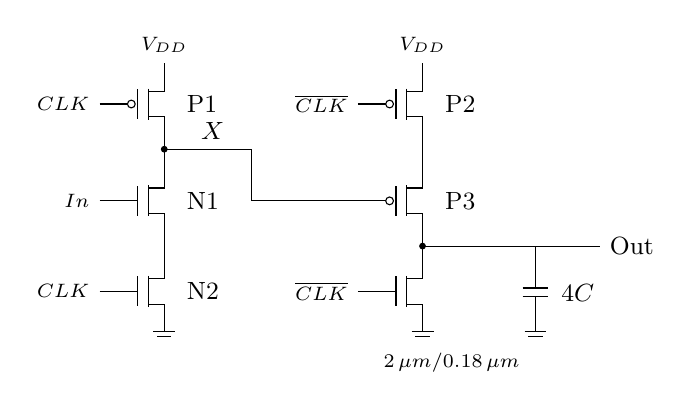
\begin{tikzpicture}[scale=.82,font=\small]
\mos{0}{3.6}{CLK}{1}\mos{0}{2.1}{In}{0}\mos{0}{.7}{CLK}{0}
\rail{.25}{4.1}{V_{DD}}\draw(.25,3.1)--(.25,2.6);\draw(.25,1.6)--(.25,1.2);\gnd{.25}{.2}
\node[right]at(.45,3.6){P1};\node[right]at(.45,2.1){N1};\node[right]at(.45,.7){N2};
\draw(.25,2.9)--(1.6,2.9)--(1.6,2.1)--(3.25,2.1);\fill(.25,2.9)circle(1.5pt);\node[above]at(1,2.9){$X$};
\mos{4}{3.6}{\overline{CLK}}{1}\mos{4}{2.1}{}{1}\mos{4}{.7}{\overline{CLK}}{0}
\rail{4.25}{4.1}{V_{DD}}\draw(4.25,3.1)--(4.25,2.6);\draw(4.25,1.6)--(4.25,1.2);\gnd{4.25}{.2}
\node[right]at(4.45,3.6){P2};\node[right]at(4.45,2.1){P3};\node[below,font=\scriptsize]at(4.7,-.1){$2\,\mu m/0.18\,\mu m$};
\draw(4.25,1.4)--(7,1.4)node[right]{Out};\fill(4.25,1.4)circle(1.5pt);
\draw(6,1.4)--(6,.75);\draw(5.8,.75)--(6.2,.75);\draw(5.8,.62)--(6.2,.62);\draw(6,.62)--(6,.2);\gnd{6}{.2}\node[right]at(6.25,.67){$4C$};
\end{tikzpicture}\\Figure 1: An NP domino logic circuit.\end{center}\newpage\textbf{2. (8 points)} Figure 2 shows a Schmitt trigger circuit, where $V_{tn}=|V_{tp}|=0.6\,V$. If you apply an input signal as shown in the left figure to the Schmitt trigger circuit, then the circuit outputs the signal as shown in the right figure. Complete the following questions.
\begin{enumerate}[label=(\alph*)]
\item Derive the ratios $\beta_{N1}/\beta_{N3}$ and $\beta_{P1}/\beta_{P3}$. (4 points)
\item In comparison with a typical inverter (i.e., without the transistors P3 and N3), is the short-circuit power of the Schmitt trigger circuit higher or smaller than that of the typical inverter? Why? (4 points)
\end{enumerate}\begin{center}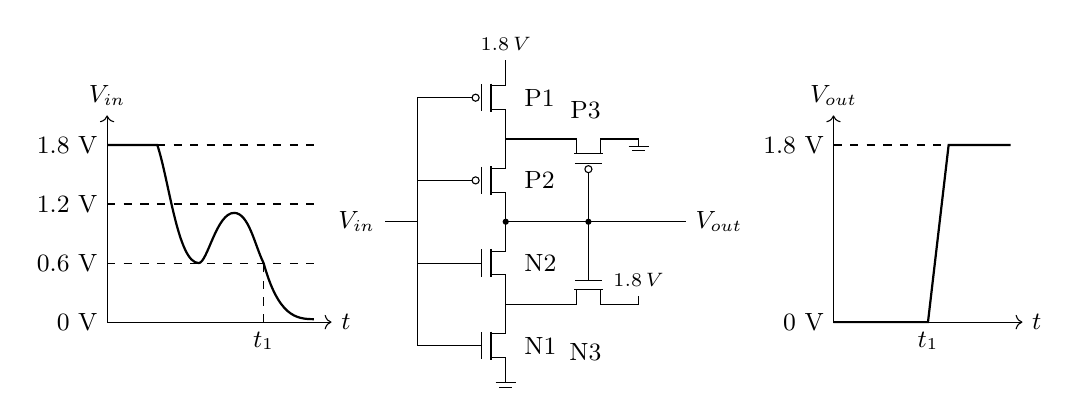
\begin{tikzpicture}[scale=.75,font=\small]
\begin{scope}[xshift=-6.5cm]
\draw[->](0,0)--(3.8,0)node[right]{$t$};\draw[->](0,0)--(0,3.5)node[above]{$V_{in}$};
\draw[dashed](0,3)--(3.5,3);\draw[dashed](0,2)--(3.5,2);\draw[dashed](0,1)--(3.5,1);
\node[left]at(0,0){0 V};\node[left]at(0,1){0.6 V};\node[left]at(0,2){1.2 V};\node[left]at(0,3){1.8 V};
\draw[thick](0,3)--(.85,3)..controls(1.05,2.4)and(1.2,1)..(1.55,1)..controls(1.7,1)and(1.85,1.85)..(2.15,1.85)..controls(2.4,1.85)and(2.5,1.3)..(2.65,1)..controls(2.9,.1)and(3.2,.05)..(3.5,.05);
\draw[dashed](2.65,0)--(2.65,1);\node[below]at(2.65,0){$t_1$};\end{scope}
\mos{0}{3.8}{}{1}\mos{0}{2.4}{}{1}\mos{0}{1}{}{0}\mos{0}{-.4}{}{0}
\rail{.25}{4.3}{1.8\,V}\draw(.25,3.3)--(.25,2.9);\draw(.25,1.9)--(.25,1.5);\draw(.25,.5)--(.25,.1);\gnd{.25}{-.9}
\draw(-.75,3.8)--(-1.25,3.8)--(-1.25,-.4)--(-.75,-.4);\draw(-1.25,2.4)--(-.75,2.4);\draw(-1.25,1)--(-.75,1);\draw(-1.25,1.7)--(-1.8,1.7)node[left]{$V_{in}$};
\node[right]at(.4,3.8){P1};\node[right]at(.4,2.4){P2};\node[right]at(.4,1){N2};\node[right]at(.4,-.4){N1};
\draw(.25,3.1)--(1.15,3.1);\begin{scope}[shift={(1.65,2.85)},rotate=90]\mos{0}{0}{}{1}\end{scope}\draw(2.15,3.1)--(2.5,3.1);\gnd{2.5}{3.1}\node[above]at(1.6,3.28){P3};
\draw(.25,.3)--(1.15,.3);\begin{scope}[shift={(1.65,.55)},rotate=-90]\mos{0}{0}{}{0}\end{scope}\draw(2.15,.3)--(2.5,.3);\rail{2.5}{.3}{1.8\,V}\node[below]at(1.6,-.2){N3};
\draw(.25,1.7)--(3.3,1.7)node[right]{$V_{out}$};\fill(.25,1.7)circle(1.5pt);\draw(1.65,2.1)--(1.65,1.3);\fill(1.65,1.7)circle(1.5pt);
\begin{scope}[xshift=5.8cm]
\draw[->](0,0)--(3.2,0)node[right]{$t$};\draw[->](0,0)--(0,3.5)node[above]{$V_{out}$};\draw[dashed](0,3)--(3,3);\node[left]at(0,0){0 V};\node[left]at(0,3){1.8 V};
\draw[thick](0,0)--(1.6,0)--(1.95,3)--(3,3);\node[below]at(1.6,0){$t_1$};\end{scope}
\end{tikzpicture}\\Figure 2: A CMOS Schmitt trigger circuit and the source waveforms.\end{center}\textbf{3. (10 points)} Figure 3 shows a domino logic gate. Assume that $0.18\,\mu m$ technology is used to design the domino logic gate and $\mu_n=2\mu_p$. Also, a $2\,\mu m/0.18\,\mu m$ PMOS/NMOS has an input gate capacitance $C$. Complete the following questions.
\begin{enumerate}[label=(\alph*)]
\item Assume that the channel length of all the transistors is $0.18\,\mu m$. If we desire to design the domino logic gate such that the switching power of the clock (CLK) is $9fCV_{dd}^2$, where $f$ and $V_{dd}$ denote the operation frequency and the power supply of the logic gate, determine the sizes of N1, N2, N3, N4, N5, N6, N7, and P1 such that the rise time and the fall time of node X are equal, i.e., $t_r=t_f$. (5 points)
\item The domino logic may have a malfunction due to leakage current when the state of X is logic 1. Modify the domino logic gate shown in Figure 3 such that it can be functionally correct. (5 points)
\end{enumerate}\begin{center}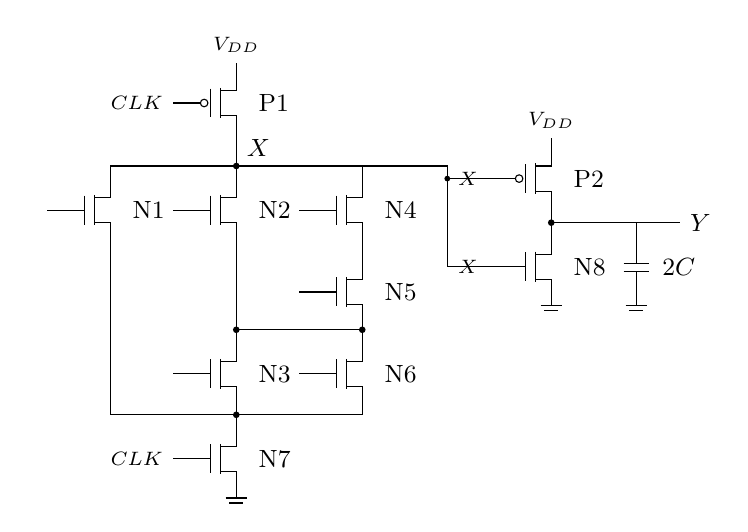
\begin{tikzpicture}[scale=.8,font=\small]
\mos{0}{5.1}{CLK}{1}\rail{.25}{5.6}{V_{DD}}\draw(.25,4.6)--(.25,4.1);\fill(.25,4.1)circle(1.5pt);\node[above]at(.6,4.1){$X$};\node[right]at(.45,5.1){P1};
\draw(-1.75,4.1)--(2.25,4.1);\mos{-2}{3.4}{}{0}\mos{0}{3.4}{}{0}\mos{2}{3.4}{}{0}\mos{2}{2.1}{}{0}\mos{0}{.8}{}{0}\mos{2}{.8}{}{0}\mos{0}{-.55}{CLK}{0}
\draw(-1.75,4.1)--(-1.75,3.9);\draw(.25,4.1)--(.25,3.9);\draw(2.25,4.1)--(2.25,3.9);\draw(2.25,2.9)--(2.25,2.6);
\draw(.25,2.9)--(.25,1.5)--(2.25,1.5);\draw(2.25,1.6)--(2.25,1.3);\draw(.25,1.5)--(.25,1.3);\fill(.25,1.5)circle(1.5pt);\fill(2.25,1.5)circle(1.5pt);
\draw(-1.75,2.9)--(-1.75,.15)--(2.25,.15);\draw(.25,.3)--(.25,-.05);\draw(2.25,.3)--(2.25,.15);\fill(.25,.15)circle(1.5pt);\gnd{.25}{-1.05}
\node[right]at(-1.55,3.4){N1};\node[right]at(.45,3.4){N2};\node[right]at(2.45,3.4){N4};\node[right]at(2.45,2.1){N5};\node[right]at(.45,.8){N3};\node[right]at(2.45,.8){N6};\node[right]at(.45,-.55){N7};
\mos{5}{3.9}{X}{1}\mos{5}{2.5}{X}{0}\rail{5.25}{4.4}{V_{DD}}\draw(5.25,3.4)--(5.25,3);\gnd{5.25}{2}\node[right]at(5.45,3.9){P2};\node[right]at(5.45,2.5){N8};
\draw(.25,4.1)--(3.6,4.1)--(3.6,2.5)--(4.25,2.5);\draw(3.6,3.9)--(4.25,3.9);\fill(3.6,3.9)circle(1.3pt);
\draw(5.25,3.2)--(7.3,3.2)node[right]{$Y$};\fill(5.25,3.2)circle(1.5pt);\draw(6.6,3.2)--(6.6,2.55);\draw(6.4,2.55)--(6.8,2.55);\draw(6.4,2.43)--(6.8,2.43);\draw(6.6,2.43)--(6.6,2);\gnd{6.6}{2}\node[right]at(6.86,2.49){$2C$};
\end{tikzpicture}\\Figure 3: A domino logic gate.\end{center}\newpage\textbf{4. (15 points)} Draw the transistor-level schematic diagrams of the two symbolic layouts shown in Figure 4.\begin{center}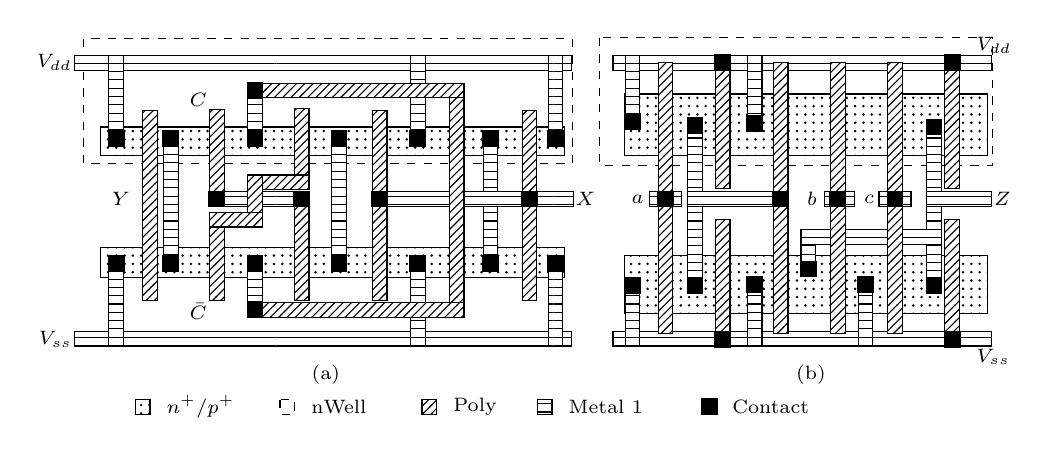
\begin{tikzpicture}[x=.011cm,y=-.011cm,font=\scriptsize]
\tikzset{lm/.style={preaction={fill=white},pattern=horizontal lines},ld/.style={preaction={fill=white},pattern=dots},lp/.style={preaction={fill=white},pattern=north east lines}}
\draw[dashed](190,30)rectangle(755,174);
\draw[dashed](786,29)rectangle(1240,176);
\draw[ld](210,132)rectangle(745,165);
\draw[ld](210,271)rectangle(745,306);
\draw[ld](815,94)rectangle(1234,165);
\draw[ld](815,280)rectangle(1234,347);
\draw[lm](179.5,49.5)rectangle(753.5,66.5);
\draw[lm](179.5,368.5)rectangle(753.5,385.5);
\draw[lm](219.5,49.5)rectangle(236.5,153.5);
\draw[lm](219.5,281.5)rectangle(236.5,385.5);
\draw[lm](282.5,136.5)rectangle(299.5,298.5);
\draw[lm](379.5,81.5)rectangle(396.5,153.5);
\draw[lm](379.5,281.5)rectangle(396.5,351.5);
\draw[lm](476.5,136.5)rectangle(493.5,298.5);
\draw[lm](567.5,49.5)rectangle(584.5,153.5);
\draw[lm](567.5,281.5)rectangle(584.5,385.5);
\draw[lm](651.5,136.5)rectangle(668.5,298.5);
\draw[lm](726.5,49.5)rectangle(743.5,153.5);
\draw[lm](726.5,281.5)rectangle(743.5,385.5);
\draw[lm](335.5,206.5)rectangle(450.5,223.5);
\draw[lm](523.5,206.5)rectangle(755.5,223.5);
\draw[lm](801.5,49.5)rectangle(1238.5,66.5);
\draw[lm](801.5,368.5)rectangle(1238.5,385.5);
\draw[lm](815.5,49.5)rectangle(832.5,134.5);
\draw[lm](815.5,306.5)rectangle(832.5,385.5);
\draw[lm](887.5,121.5)rectangle(904.5,323.5);
\draw[lm](887.5,206.5)rectangle(1003.5,223.5);
\draw[lm](956.5,49.5)rectangle(973.5,136.5);
\draw[lm](956.5,305.5)rectangle(973.5,385.5);
\draw[lm](1084.5,305.5)rectangle(1101.5,385.5);
\draw[lm](1163.5,123.5)rectangle(1180.5,323.5);
\draw[lm](1018.5,250.5)rectangle(1035.5,304.5);
\draw[lm](1018.5,250.5)rectangle(1180.5,267.5);
\draw[lm](1163.5,206.5)rectangle(1238.5,223.5);
\draw[lm](843.5,206.5)rectangle(880.5,223.5);
\draw[lm](1045.5,206.5)rectangle(1080.5,223.5);
\draw[lm](1108.5,206.5)rectangle(1145.5,223.5);
\draw[lp](258.5,112.5)rectangle(275.5,332.5);
\draw[lp](335.5,111.5)rectangle(352.5,223.5);
\draw[lp](335.5,230.5)rectangle(352.5,332.5);
\draw[lp](433.5,110.5)rectangle(450.5,204.5);
\draw[lp](379.5,187.5)rectangle(450.5,204.5);
\draw[lp](379.5,187.5)rectangle(396.5,247.5);
\draw[lp](335.5,230.5)rectangle(396.5,247.5);
\draw[lp](433.5,206.5)rectangle(450.5,332.5);
\draw[lp](523.5,112.5)rectangle(540.5,332.5);
\draw[lp](612.5,81.5)rectangle(629.5,351.5);
\draw[lp](379.5,81.5)rectangle(629.5,98.5);
\draw[lp](379.5,334.5)rectangle(629.5,351.5);
\draw[lp](696.5,112.5)rectangle(713.5,332.5);
\draw[lp](853.5,57.5)rectangle(870.5,370.5);
\draw[lp](919.5,49.5)rectangle(936.5,203.5);
\draw[lp](919.5,238.5)rectangle(936.5,385.5);
\draw[lp](986.5,57.5)rectangle(1003.5,370.5);
\draw[lp](1052.5,57.5)rectangle(1069.5,370.5);
\draw[lp](1118.5,57.5)rectangle(1135.5,370.5);
\draw[lp](1184.5,49.5)rectangle(1201.5,203.5);
\draw[lp](1184.5,238.5)rectangle(1201.5,385.5);
\draw[fill=black](219,136)rectangle(237,154);
\draw[fill=black](219,281)rectangle(237,299);
\draw[fill=black](282,136)rectangle(300,154);
\draw[fill=black](282,281)rectangle(300,299);
\draw[fill=black](379,81)rectangle(397,99);
\draw[fill=black](379,136)rectangle(397,154);
\draw[fill=black](379,281)rectangle(397,299);
\draw[fill=black](379,334)rectangle(397,352);
\draw[fill=black](476,136)rectangle(494,154);
\draw[fill=black](476,281)rectangle(494,299);
\draw[fill=black](567,136)rectangle(585,154);
\draw[fill=black](567,281)rectangle(585,299);
\draw[fill=black](651,136)rectangle(669,154);
\draw[fill=black](651,281)rectangle(669,299);
\draw[fill=black](726,136)rectangle(744,154);
\draw[fill=black](726,281)rectangle(744,299);
\draw[fill=black](335,206)rectangle(353,224);
\draw[fill=black](433,206)rectangle(451,224);
\draw[fill=black](523,206)rectangle(541,224);
\draw[fill=black](696,206)rectangle(714,224);
\draw[fill=black](815,117)rectangle(833,135);
\draw[fill=black](815,306)rectangle(833,324);
\draw[fill=black](887,121)rectangle(905,139);
\draw[fill=black](887,306)rectangle(905,324);
\draw[fill=black](956,119)rectangle(974,137);
\draw[fill=black](956,305)rectangle(974,323);
\draw[fill=black](1084,305)rectangle(1102,323);
\draw[fill=black](1163,123)rectangle(1181,141);
\draw[fill=black](1163,306)rectangle(1181,324);
\draw[fill=black](1018,287)rectangle(1036,305);
\draw[fill=black](853,206)rectangle(871,224);
\draw[fill=black](986,206)rectangle(1004,224);
\draw[fill=black](1052,206)rectangle(1070,224);
\draw[fill=black](1118,206)rectangle(1136,224);
\draw[fill=black](919,49)rectangle(937,67);
\draw[fill=black](919,368)rectangle(937,386);
\draw[fill=black](1184,49)rectangle(1202,67);
\draw[fill=black](1184,368)rectangle(1202,386);
\node[left]at(188,58){$V_{dd}$};\node[left]at(188,377){$V_{ss}$};\node[left]at(255,215){$Y$};\node[above left]at(344,120){$C$};\node[below left]at(344,324){$\bar C$};\node[right]at(747,215){$X$};
\node[above right]at(1210,58){$V_{dd}$};\node[below right]at(1210,377){$V_{ss}$};\node[left]at(848,215){$a$};\node[left]at(1048,215){$b$};\node[left]at(1114,215){$c$};\node[right]at(1230,215){$Z$};
\node at(470,418){(a)};\node at(1030,418){(b)};
\draw[ld](250,447)rectangle(267,464);
\node[right]at(275,455){$n^+/p^+$};
\draw[dashed](417,447)rectangle(434,464);
\node[right]at(442,455){nWell};
\draw[lp](581,447)rectangle(598,464);
\node[right]at(606,455){Poly};
\draw[lm](714,447)rectangle(731,464);
\node[right]at(739,455){Metal 1};
\draw[fill=black](904,446)rectangle(922,464);
\node[right]at(928,455){Contact};
\end{tikzpicture}\\Figure 4: Symbolic layouts of two circuits.\end{center}\textbf{5. (15 points)} Figure 5 shows a sequential circuit. Assume that the clock-to-Q propagation delay ($t_{pcq}$), the clock-to-Q contamination delay ($t_{ccq}$), the setup time ($t_{setup}$), and the hold time ($t_{hold}$) of the registers are $0.3\,ns$, $0.1\,ns$, $0.3\,ns$, and $0.4\,ns$, respectively. The delay of the NOR gate, the XOR gate, the XNOR gate, and the inverter is $0.3\,ns$, $0.5\,ns$, $0.4\,ns$, and $0.2\,ns$, respectively. Also, the delay of interconnection between R1 and R4 is $0.1\,ns$. Complete the following questions.
\begin{enumerate}[label=(\alph*)]
\item Can the circuit be operated correctly? If not, how do you modify the circuit by inserting additional logic gates (e.g., the NOR gate, XNOR gate, or the inverter shown above) such that it can operate correctly without sacrifice of the operation frequency? Draw the modified circuit. (6 points)
\item Determine the maximum operation frequency of the circuit. (4 points)
\item If the clock skew is $0.5\,ns$, determine the maximum operation frequency of the sequential circuit. (5 points)
\end{enumerate}\begin{center}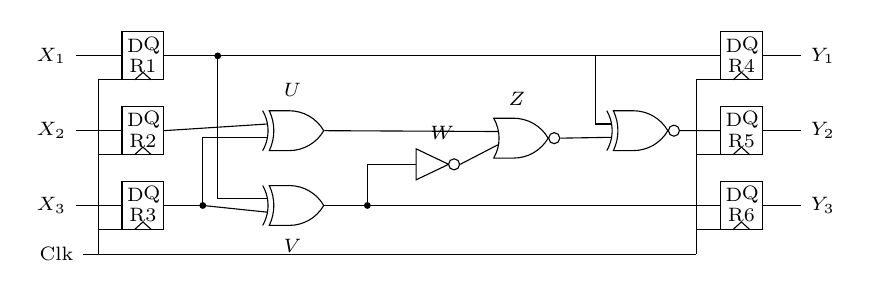
\begin{tikzpicture}[scale=.95,font=\scriptsize]
\draw(-0.28,1.68)rectangle(0.28,2.32);\node at(-0.1,2.14){D};\node at(0.12,2.14){Q};\node at(0,1.87){R1};
\draw(-0.11,1.68)--(0,1.78)--(0.11,1.68);
\draw(-0.28,2)--(-.9,2)node[left]{$X_{1}$};
\draw(-0.28,0.6799999999999999)rectangle(0.28,1.32);\node at(-0.1,1.1400000000000001){D};\node at(0.12,1.1400000000000001){Q};\node at(0,0.87){R2};
\draw(-0.11,0.6799999999999999)--(0,0.78)--(0.11,0.6799999999999999);
\draw(-0.28,1)--(-.9,1)node[left]{$X_{2}$};
\draw(-0.28,-0.32)rectangle(0.28,0.32);\node at(-0.1,0.14){D};\node at(0.12,0.14){Q};\node at(0,-0.13){R3};
\draw(-0.11,-0.32)--(0,-0.22)--(0.11,-0.32);
\draw(-0.28,0)--(-.9,0)node[left]{$X_{3}$};
\draw(7.72,1.68)rectangle(8.28,2.32);\node at(7.9,2.14){D};\node at(8.12,2.14){Q};\node at(8,1.87){R4};
\draw(7.89,1.68)--(8,1.78)--(8.11,1.68);
\draw(8.28,2)--(8.8,2)node[right]{$Y_{1}$};
\draw(7.72,0.6799999999999999)rectangle(8.28,1.32);\node at(7.9,1.1400000000000001){D};\node at(8.12,1.1400000000000001){Q};\node at(8,0.87){R5};
\draw(7.89,0.6799999999999999)--(8,0.78)--(8.11,0.6799999999999999);
\draw(8.28,1)--(8.8,1)node[right]{$Y_{2}$};
\draw(7.72,-0.32)rectangle(8.28,0.32);\node at(7.9,0.14){D};\node at(8.12,0.14){Q};\node at(8,-0.13){R6};
\draw(7.89,-0.32)--(8,-0.22)--(8.11,-0.32);
\draw(8.28,0)--(8.8,0)node[right]{$Y_{3}$};
\node[xor gate US,draw,logic gate inputs=nn](u)at(2,1){};\node[xor gate US,draw,logic gate inputs=nn](v)at(2,0){};
\node[not gate US,draw](w)at(3.8,.55){};\node[nor gate US,draw,logic gate inputs=nn](z)at(5.0,.9){};\node[xnor gate US,draw,logic gate inputs=nn](g)at(6.6,1){};
\draw(.28,1)--(u.input 1);\draw(.28,0)--(.8,0)|-(u.input 2);\draw(.8,0)--(v.input 2);\fill(.8,0)circle(1.3pt);
\draw(.28,2)--(1.0,2);\draw(1.0,2)|-(v.input 1);\fill(1.0,2)circle(1.3pt);
\draw(u.output)--(z.input 1);\draw(v.output)--(3,0);\draw(3,0)|-(w.input);\draw(w.output)--(z.input 2);\draw(z.output)--(g.input 2);
\draw(1.0,2)--(6.05,2)|-(g.input 1);\draw(g.output)--(7.72,1);\draw(3,0)--(7.72,0);\fill(3,0)circle(1.3pt);
\node[above]at(2,1.32){$U$};\node[below]at(2,-.32){$V$};\node[above]at(4,.75){$W$};\node[above]at(5,1.2){$Z$};
\draw(1.0,2)--(7.72,2);
\draw(-.8,-.65)--(7.4,-.65);\node[left]at(-.8,-.65){Clk};\draw(-.6,-.65)--(-.6,1.68);\draw(7.4,-.65)--(7.4,1.68);\draw(-.6,-.32)--(0,-.32);\draw(-.6,.68)--(0,.68);\draw(-.6,1.68)--(0,1.68);\draw(7.4,-.32)--(8,-.32);\draw(7.4,.68)--(8,.68);\draw(7.4,1.68)--(8,1.68);
\end{tikzpicture}\\Figure 5: A sequential circuit.\end{center}\newpage\textbf{6. (10 points)} Figure 6 shows one possible implementation of the D register. Complete the following questions.
\begin{enumerate}[label=(\alph*)]
\item Figure 6 shows a register consisting of a master latch and a low-cost slave latch. Assume that the delay of Inv1, Inv2, and the transmission gate is $0.2\,ns$, $0.2\,ns$, and $0.1\,ns$, respectively. Define the setup time of the register if the clock is ideal. (4 points)
\item As Figure 6 shows, assume that the switching threshold voltage of Inv2 is $V_{dd}/2$, and the turn-on equivalent resistances of the transmission gate, N1, N2, P1, and P2 are $R_{TS}$, $R_{N1}$, $R_{N2}$, $R_{P1}$, and $R_{P2}$, respectively. List two inequalities for determining the sizes of P2 and N2 such that the register can be operated correctly. (6 points)
\end{enumerate}\begin{center}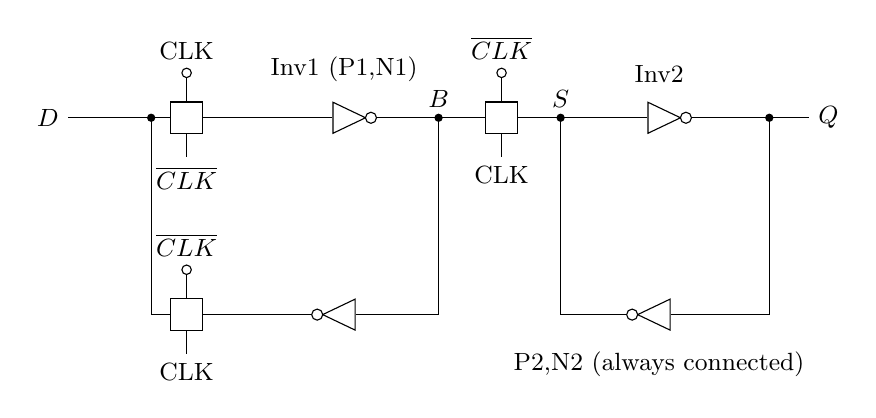
\begin{tikzpicture}[scale=1,font=\small]
\draw(-.5,1.5)--(.8,1.5)node[pos=0,left]{$D$};\draw(.8,1.3)rectangle(1.2,1.7);\draw(1,1.7)--(1,2.0);\draw(1,2.07)circle(.06);\node[above]at(1,2.12){CLK};\draw(1,1.3)--(1,1.0)node[below]{$\overline{CLK}$};
\node[not gate US,draw](i1)at(3,1.5){};\node[above]at(3,1.83){Inv1 (P1,N1)};\draw(1.2,1.5)--(i1.input);\draw(i1.output)--(4.8,1.5);\node[above]at(4.2,1.5){$B$};
\draw(.8,-1.2)rectangle(1.2,-.8);\draw(1,-.8)--(1,-.5);\draw(1,-.43)circle(.06);\node[above]at(1,-.38){$\overline{CLK}$};\draw(1,-1.2)--(1,-1.5)node[below]{CLK};
\draw(.8,-1.0)--(.55,-1.0)--(.55,1.5);\fill(.55,1.5)circle(1.5pt);\node[not gate US,draw,rotate=180](ifb)at(3,-1.0){};\draw(ifb.output)--(1.2,-1.0);\draw(ifb.input)--(4.2,-1.0)--(4.2,1.5);\fill(4.2,1.5)circle(1.5pt);
\draw(4.8,1.3)rectangle(5.2,1.7);\draw(5,1.7)--(5,2.0);\draw(5,2.07)circle(.06);\node[above]at(5,2.12){$\overline{CLK}$};\draw(5,1.3)--(5,1.0)node[below]{CLK};
\node[not gate US,draw](i2)at(7,1.5){};\node[above]at(7,1.83){Inv2};\draw(5.2,1.5)--(i2.input);\draw(i2.output)--(8.9,1.5)node[right]{$Q$};
\node[not gate US,draw,rotate=180](isfb)at(7,-1.0){};\node[below]at(7,-1.35){P2,N2 (always connected)};\draw(isfb.input)--(8.4,-1.0)--(8.4,1.5);\fill(8.4,1.5)circle(1.5pt);\draw(isfb.output)--(5.75,-1.0)--(5.75,1.5);\fill(5.75,1.5)circle(1.5pt);\node[above]at(5.75,1.5){$S$};
\end{tikzpicture}\\Figure 6: A static register. Each inverter symbol denotes its CMOS pMOS/nMOS pair.\end{center}\textbf{7. (12 points)} Sketch the Boolean function $f=\overline{(A+BC)D}$ using each of the following logic design techniques: (1) Dynamic logic (4 points) (2) Fully differential logic (4 points) (3) Differential split-level logic (4 points).\par\medskip\textbf{8. (30 points)} Answer the following questions.
\begin{enumerate}[label=(\alph*)]
\item List two approaches which can be used to alleviate the occurrence probability of latchup. (4 points)
\item List two requirements which must be met when you draw the layout of a cell in the standard cell library. (4 points)
\item Why is the soft error rate of a circuit increased with increasing operation frequency and scaling down the technology process? Explain the cause in terms of the logical masking effect, electrical masking effect, and latch window effect. (6 points)
\item List two methods to reduce the power bounce and ground bounce occurring in the IO pads. (4 points)
\item List two major problems of dynamic logic. (4 points)
\item List two limitations of CMOS domino logic. (4 points)
\item What are core-limited design and pad-limited design? (4 points)
\end{enumerate}\end{document}